\appendix
%\section{Appendices}
\label{sec:appendix}
%\subsection{Appendix A}
%\label{app:md-data}

%We begin with $n$ data points of dimension $3N_a$ corresponding to the Euclidean coordinates of each atom within the molecule. To respect rotational, dilation, and translational molecular symmetry, we transform these $3N_a$ coordinates into $D= 3 {N_a \choose 3}$ angles of atomic triplets. These coordinates are then used to learn an embedding in m coordinates.

%\ouralg~ is applied to a randomly chosen subset of $n'$ using $p$ dictionary functions, and this process is repeated reps number of times. Importantly, since our angular coordinates are redundant, we necessarily adapt \ouralg~ to the shape space $\Sigma_3^{N_a}$. Embedding and tangent space estimation is done in dimension $D$, while normalization and regression is done in the shape space of dimension $3N_a - 7$. In all experiments, we assume that manifold dimension $d$ has already been estimated. The full specifics of our MD data analytics pipeline are in Appendix \ref{app:md-data}.


%This section describes details of the data processing. Sections \ref{sec:}--\ref{sec:} describes the experimental results. In both 'real' and synthetic MD experiments our data processing procedure procedure is as follows. \mmp{samples, transformatin and preprocessing, manifold embedding -- what alg and params, manifold lasso}


%We consider a molecular position to be a collection of $N_a$ points in $\mathbb R^3$, where $N_a$ is the number of atoms in the molecule. A molecular trajectory consists of a set or sequence of molecular positions. We apply a manifold learning algorithm to identify the low-dimensional manifold these trajectories are sampled around. We then apply \ouralg~  to perform sparse functional support recovery for the embedding coordinates. In particular, we identify an explanation of this manifold in terms of bond torsions.
%\subsection{Appendix B}

\section{The shape space}
\label{app:shape-space}
Here we formally define the shape space, and show how to obtain the gradient of a function $g_j$ of a molecular configuration, at a non-singular point, in the tangent bundle of this space.

We define the \textit{shape space}
\begin{align*}
 \Sigma_3^{N_a} = \rrr^{3N_a} \slash (E(3) \times \rrr^+ ),
\end{align*}
where $E(3)$ is the three dimensional Euclidean group composed of rigid rotations and translations in $\rrr^3$, and $\rrr^+$ is a dilation factor relative to the mean position of the $N_a$ atoms. That is, $\Sigma_3^{N_a}$ is the space of positions of $N_a$ atoms in $\rrr^3$ with equivalences given by translation, rotation, and dilation. Away from singularities of measure zero, $\Sigma_3^{N_a}$ is a Riemannian manifold \citep{Le1993-mg, addicoatcollins:2010}.

Denote the Euclidean coordinates of $ \rrr^{3N_a}$ by $r$, and the Euclidean position of each data point by $r_i$. Recall that we compute $a_i = a(r_i)$ for $i \in 1, \dotsc n$, where $a$ is the vector-valued function
\begin{align*}
a: \rrr^{3N_a} \to \rrr^{3{N_a \choose 3}}
\end{align*}
that computes the angles formed by all triples of atoms in the molecule. This angular featurization of the data respects the symmetries of the shape space, and embeds the shape space.
%\label{sec:test}
We compute bases for the tangent spaces of $\Sigma_3^{N_a}$ as follows. For every analyzed point $i$, we compute the matrix of partial derivatives, also known as the Wilson B-matrix,
\begin{align*}
W_i = \frac{\partial a}{\partial r} (r_i) \in \mathbb R^{3N_a \times \mathbb R^{3 {N_a \choose 3}}}.
\end{align*}
Note that $W_i$ is the transpose Jacobian of $a$. 
%Away from singularities of measure zero, we can compute the tangent space of $\Sigma_3^{N_a}$ with respect to its embedding in $\rrr^{3{N_a \choose 3}}$. By projecting onto $T \Sigma_3^{N_a}$, we remove the issue of angular redundancy in the sense that all gradients of the same torsion are equivalent after projection, regardless of which angles were used to compute the torsion. Thus, normalization with respect to these gradients is well-defined.
This computation is done using automatic differentiation. We then calculate the reduced Singular Value Decomposition
\begin{align*}
W_i = U_i \Lambda_i V_i^T
\end{align*}
where  $\Lambda_i$ is a diagonal matrix of dimension $3N_a - 7$, containing the non-zero singular values of $W_i$. A deductive explanation for the rank of $W_i$ is that translation, rotation, and dilation correspond to a total of 7 degrees of freedom. The $3N_a - 7$ corresponding singular vectors in $V_i$ are a basis for the tangent space $\T_i  \Sigma_3^{N_a}$ in $\rrr^{3 {N_a \choose 3}}$ \citep{addicoatcollins:2010}. Let $a_i = a(r_i)$ for $i \in 1, \dotsc n$. We can then project
\begin{align*}
%\grad_{\Sigma_3^{N_a}} g_j (a_i) &= V_i V_i^T \nabla_{\mathbb R^{3 {N_a \choose 3}}} g_j (a_i),
\grad_{\Sigma_3^{N_a}} g_j (a_i) &= V_i V_i^T \nabla_{a} g_j (a_i),
\end{align*}
where $\nabla_a g_j (a_i)$ is obtained with automatic differentiation using a close-form expression for the dictionary function in the angular coordinates $a$ of $\rrr^{3 {N_a \choose 3}}$, and $\grad_{\Sigma_3^{N_a}}$ is the gradient on the shape manifold in the angular coordinates.

Recall that we apply Principal Component Analysis to the angular features matrix  $a_{1:n} \in \rrr^{n \times D}$. To perform PCA, we use Singular Value Decomposition:
\begin{align*}
a_{1:n} = M \Pi N^T.
\end{align*}
Denote by $P$ the matrix formed with the first $D$ columns of $N$; $P$ projects the angular features into a lower dimension space that reduces redundancy while capturing the vast majority of the variability. \comment{For this paper, we use $D = 50$.} That is, \\
\begin{align*}
\xi_i &= a_i P,\;\text{for}\; i=1,\ldots n.
\end{align*}
The gradient of $g_j$ with respect to coordinates $\xi$ are given by
\begin{align*}
\grad_{\xi} g_j (\xi_i)= P^T \grad_{\Sigma_3^{N_a}} g_j (a_i).
\end{align*}
We use $\grad_{\xi} g_j (\xi_i)$ as $\nabla_{\xi} g_j (\xi_i)$ in \ouralg.
%We then normalize with respect to $\grad_{\xi} g_j$.
%\begin{align*}
%\grad_{\xi} g_j (\xi_i) =\frac{ \grad_{PCA} g_j (\xi_i)}{\sum_{i=1}^n \| \grad_{\xi} g_j (\xi_i) \|_2}
%\end{align*}
%Finally, we compute
%\begin{align*}
%TM^T \grad_{\xi} g_j = \grad_{M} g_j.
%\end{align*}
%We utilize $\grad_{\Sigma_3^{N_a}} \phi_m$ and the normalized version of $\grad_{\Sigma_3^{N_a}} g_j$ as our functional variables in group lasso.

%That is, $ respect this symmetry, we featurize each configuration in terms of the angles of the triangles formed by all combinations of three atoms, i.e. as an element of $\rrr^D$, where $D = 3{N_a \choose 3}$. The manifold learning algorithm is then applied to this representation of the data.

%In order for our normalization procedure to be well-defined, it is necessary to consider the dictionary functions as functions of the manifold $\Sigma_3^{N_a}$ rather than $\rrr^D$. This is because $\rrr^D$ is an overparameterized space, and so dictionary functions do not have a unique gradient field. To remedy this, we project any suitable gradient field computed in $\rrr^D$ onto the tangent bundle of $\Sigma_3^{N_a}$. This projection is based on the idea that $\Sigma_3^{N_a}$ is a rank $3N_a - 7$ space inside of $\rrr^D$, and amounts to identifying the tangent bundle of $\Sigma_3^{N_a}$ using differential constraints between the angles. Although this space has singularities, they are of measure zero, and are not encountered in practice. Note that we cannot apply an embedding algorithm to $\Sigma_3^{N_a}$ directly, since this is not a Euclidean space, and nearest neighbor search is not guaranteed to be work, although in principle we could search in $\rrr^D$ and compute geometry with respect to $\Sigma_3^{N_a}$. Also note that the metric we implicitly use for $\Sigma_3^{N_a}$ is inherited from the angular representation, therefore that our shape space is not isometric to that of \cite{le}.

%\mmp{Shape space thoughts> Let $a$ be the angle coordinates, $\xi$ be the coordinates obtained from $a$ after PCA, and $r$ be the Cartesian atom coordinates. We have that $\xi=\sqrt{\Sigma}U^Ta$, where $Cov(a)=U\Sigma U^T$, and $\Sigma$ has rank $D$. Then, $\fracpartial{\xi}{r}=\sqrt{\Sigma}U^T\fracpartial{a}{r}$, with $\fracpartial{a}{r}$ obtained by automatic differentiation. We calculate the SVD of $\fracpartial{\xi}{r}$,
%\[
%\fracpartial{\xi}{r}\;=\;U_\xi\Lambda_\xi V_\xi^T
%\]
%where  $\Lambda$ contains $3N_a - 7$ non-zero eigenvalues. The first $3N_a - 7$ eigenvectors in $U_\xi$ are a basis for the tangent space $\T \tilde \Sigma_3^{N_a}$ embedded in $\rrr^D$. We can then project the gradients of $g_j$ obtained by automatic differentiation w.r.t. $r$ onto this tangent space by
%\[
%\grad_\xi g_j\;=\;U_\xi\nabla_r g_j
%\]
%We use $\grad_\xi g_j$ in place of $\nabla_\xi g_j$ in the \ouralg~algorithm.
%}

%\skcomment{I believe it is a different idea. The core of the idea may be preferable to what we are currently doing, but I am not sure.  Here is a major point of confusion for me (using your notation): 
%$\frac{\partial \xi}{\partial r} \in \mathbb R^{3N_a \times  D}$
%so if $\frac{\partial \xi}{\partial r} = U_\xi \lambda_\xi V_\xi^T$
%then the first $3N_a - 7$ singular vectors of $U_\xi$ form a matrix $\tilde U_\xi \in \mathbb R^{3N_a \times 3N_a-7}.$
%Then we get $\tilde U_\xi^T \nabla_r g_j \in \mathbb R^{3N_a-7} \neq \mathbb R^D.$
%So I don't think the dimensions of the vectors are what we are looking for.
%There may be a similar approach taking advantage of the fact that $\frac{\partial \xi}{\partial r}$ is rank $3N_a-7$.}

\begin{figure}[H]
\setlength{\picwi}{0.3\llw}
\begin{tabular}{cc} 
%A
%\includegraphics[width=1.5\picwi,height=2\picwi]{rigapp.png}
% &
%B
%\includegraphics[width=1.5\picwi,height=2\picwi]{rigbpp.png} \\
%\multicolumn{2}{c}{
%C
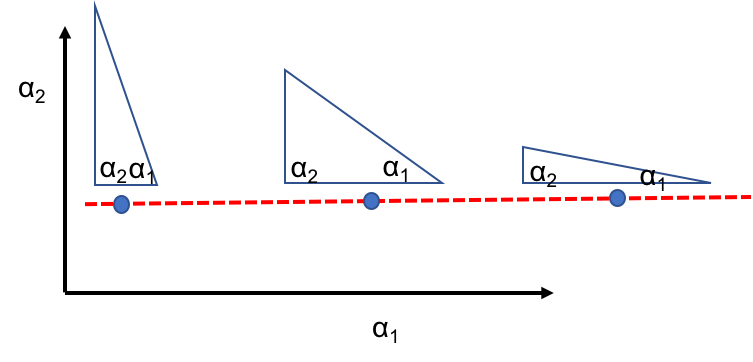
\includegraphics[width=4\picwi,height=2\picwi]{../Figures/righttriangles.png}
\end{tabular}
\caption{\label{fig:shapespace} This diagram shows a simplified representation of the neighborhood of a point in the shape space $\Sigma_2^3$. Up to rotation, dilation, and translation, the shape of a triangle is determined by two angles, so we can see that this is a two-dimensional space.  The diagram represents the logarithmic map of a region of $\Sigma_2^3$, with the red line indicating the logarithmic map of the subspace of right triangles, in a coordinate system given by $\alpha_1$ and $\alpha_2$, two angles in the triangle.
}
\end{figure}

%<<<<<<< HEAD


%\subsection{Appendix B}
%\label{app:function-dependency-data}

%\subsection{Appendix C}
%\label{app:embedding-algorithm}
%=======
%At every data point, denote the basis of $D$ redundant angular variables by $z$, and the $3N_a$ Euclidean coordinates of the molecule by $x$. For every analyzed point, we compute the matrix of partial derivatives, also known as the Wilson B-matrix,
%\begin{align*}
%W = \frac{\partial z}{\partial x}.
%\end{align*}
%When then perform a singular value decomposition
%\begin{align*}
%W = U \Lambda U^T
%\end{align*}
%where  $\Lambda$ contains $3N_a - 7$ non-zero eigenvalues. A deductive explanation for the rank of $W$ is that translation, rotation, and dilation correspond to a total of 7 degrees of freedom. The first $3N_a - 7$ eigenvectors in $U$ are a basis for the tangent space $T \tilde \Sigma_3^{N_a}$ embedded in $\rrr^D$. We can then project
%\begin{align*}
%\grad_{\Sigma_3^{N_a}} g_j &= U \grad_D g_j \; \text {and} \\
%\grad_{\Sigma_3^{N_a}} \phi_m &= U \grad_{D} \phi_m. \text{\mmp{we don't do this, right?}}
%\end{align*}
%We utilize $\grad_{\Sigma_3^{N_a}} \phi_m$ and the normalized version of $\grad_{\Sigma_3^{N_a}} g_j$ as our functional variables in group lasso.

%\section{Function dependency data}
%\label{app:function-dependency-data}
%\mmp{what's this?}
%\section{Diffusion Maps embedding algorithm}
%\label{app:embedding-algorithm}
%>>>>>>> cdd11cc241cb349bd809fb501520a4e91935eb18

\section{Torsion Computation}
\label{app:dictionary-details}

For molecular dynamics analyses, our dictionary $\G$ consists of bond torsions, which are computed from angles, and whose gradients are obtained using automatic differentiation in Pytorch.
  Diagrams \ref{figtab:eth} -  \ref{figtab:mal} show the identities of the torsions input as functional dictionaries to \ouralg.  Torsions experimentally validated to explain the data manifold are marked with a *.
  
\begin{table}[H]
\begin{tabular}{cc}
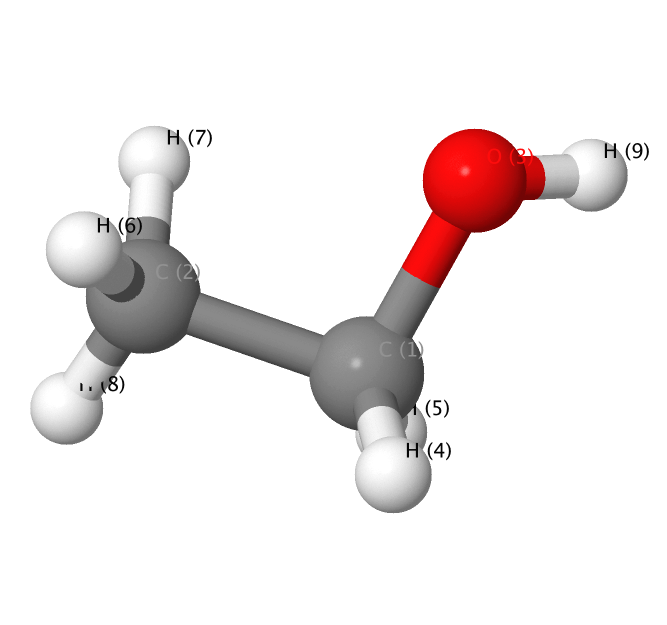
\includegraphics[scale=0.25,valign=m]{../Figures/ethanol/ethanol.png}
&
\begin{tabular}{ | c | c | } 
\hline
\G \# & Atom \# s \\
\hline
$g_1*$ & [7,2,1,5]\\
\hline
$g_2*$ & [5,1,3,9] \\
\hline
$g_3$ & [8,7,6,2] \\
\hline
$g_4$ & [4,1,3,5]\\
\hline
\end{tabular}
\end{tabular}
\caption{Diagram of ethanol and identities of bond torsions.  Torsions are the angle of the planes formed by the first three and last three atoms. Torsions experimentally validated to explain the data manifold are marked with a *.}
\label{figtab:eth}
\end{table}
%\clearpage

%\FloatBarrier
%\paragraph{Toluene}

\begin{table}[hbt!]
\begin{tabular}{cc}
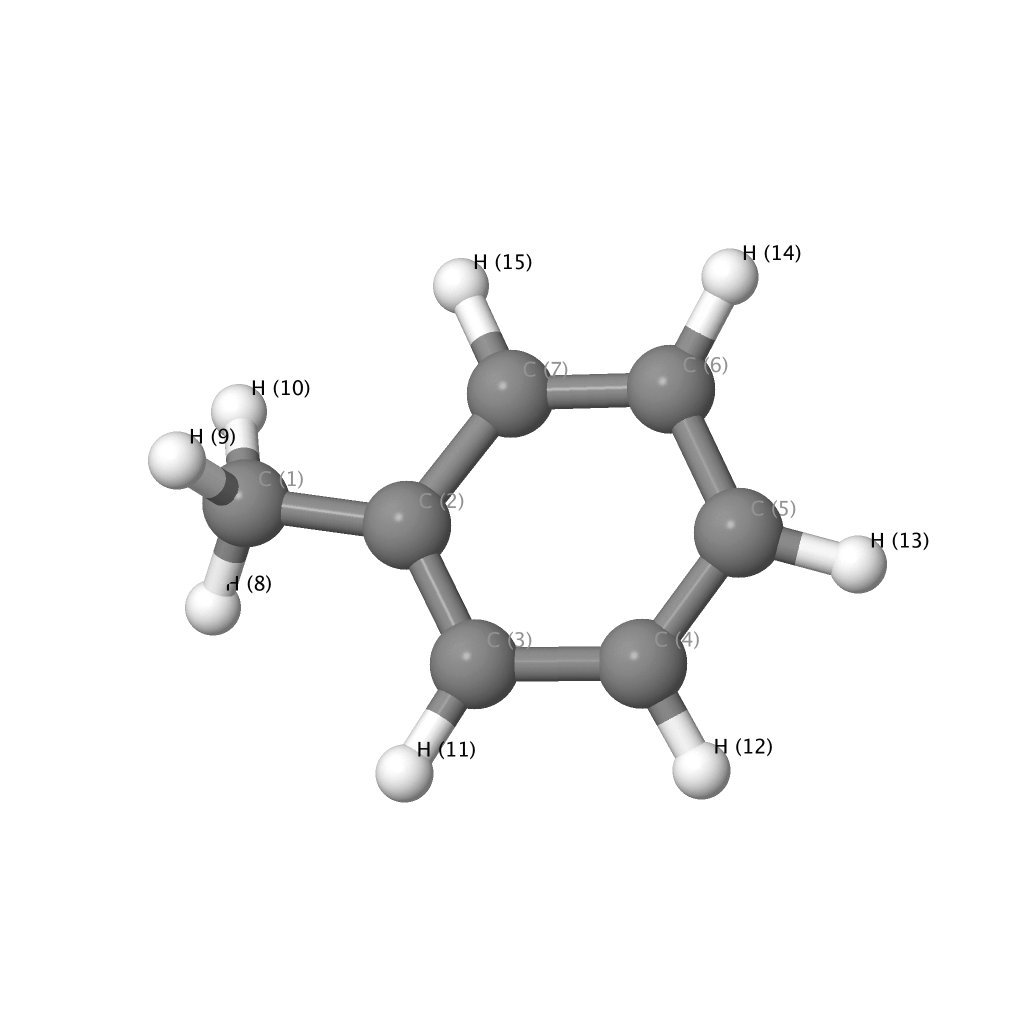
\includegraphics[scale=0.25,valign=m]{../Figures/toluene/toluene.png}
&
\begin{tabular}{ | c | c | } 
\hline
Torsion \# & Atom \# s \\
\hline
$g_1*$ & [10,1,2,3]\\
\hline
$g_2$ & [1,2,3,4]\\
\hline
$g_3$ &[2,3,4,5]\\
\hline
$g_4$ & [3,4,5,6]\\
\hline
$g_5$ &[4,5,6,7]\\
\hline
$g_6$ &[5,6,7,2]\\
\hline
$g_7$ &[6,7,2,1]\\
\hline
$g_8$ & [1,2,4,12] \\
\hline
$g_9$  & [11,3,5,13]  \\
\hline 
$g_{10}$ & [12,4,6,14] \\
\hline 
$g_{11}$ & [13,5,7,15] \\
\hline 
$g_{12}$ & [11,3,7,14] \\
\hline 
$g_{13}$ & [1,2,6,14] \\
\hline 
$g_{14}$ & [12,4,7,15] \\
\hline 
$g_{15}$ & [13,5,2,1] \\
\hline 
$g_{16}$ & [11,3,6,14] \\
\hline
\end{tabular}
\end{tabular}
\caption{Diagram of toluene and identities of bond torsions.  Torsions are the angle of the planes formed by the first three and last three atoms. Torsions experimentally validated to explain the data manifold are marked with a *.}
\label{figtab:tol}
\end{table}

%\paragraph{Malonaldehyde}


\begin{table}[hbt!]
\begin{tabular}{cc}
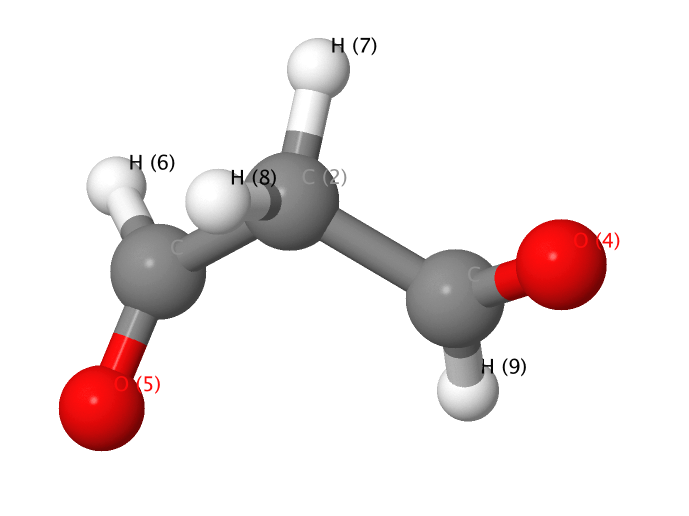
\includegraphics[scale=0.25,valign=m]{../Figures/malonaldehyde/malonaldehyde.png}
&
\begin{tabular}{ | c | c | } 
\hline
$\G$ \# & Atom \# s \\
\hline
$g_1*$ & [5,1,2,3]\\
\hline
$g_2*$ &[1,2,3,4]\\
\hline
$g_3$ &[4,3,2,9]\\
\hline
$g_4$ &[5,1,2,6] \\
\hline
\end{tabular}
\end{tabular}
\caption{Diagram of malonaldehyde and identities of bond torsions.  Torsions are the angle of the planes formed by the first three and last three atoms. Torsions experimentally validated to explain the data manifold are marked with a *.}
\label{figtab:mal}
\end{table}

%}
%\end{figure}
